\documentclass[ngerman]{fbi-aufgabenblatt}

\usepackage{amsmath}
\usepackage{amssymb}
\usepackage{verbatim}
\usepackage{tikz}

% Folgende Angaben bitte anpassen

\renewcommand{\Vorlesung}{Grundlagen der Wissensverarbeitung}
\renewcommand{\Semester}{WiSe 17/18}

\renewcommand{\Aufgabenblatt}{9}
\renewcommand{\Teilnehmer}{ Übungsgruppe 2; Tom Kastek (4kastek@inf), Phil Sehlmeyer (4sehlmey@inf), Max Wutz (wutzmax@googlemail.com)}

\begin{document}

\aufgabe{Exercise 9.3: (Diagnosis (cont.))}

Belief Network\\

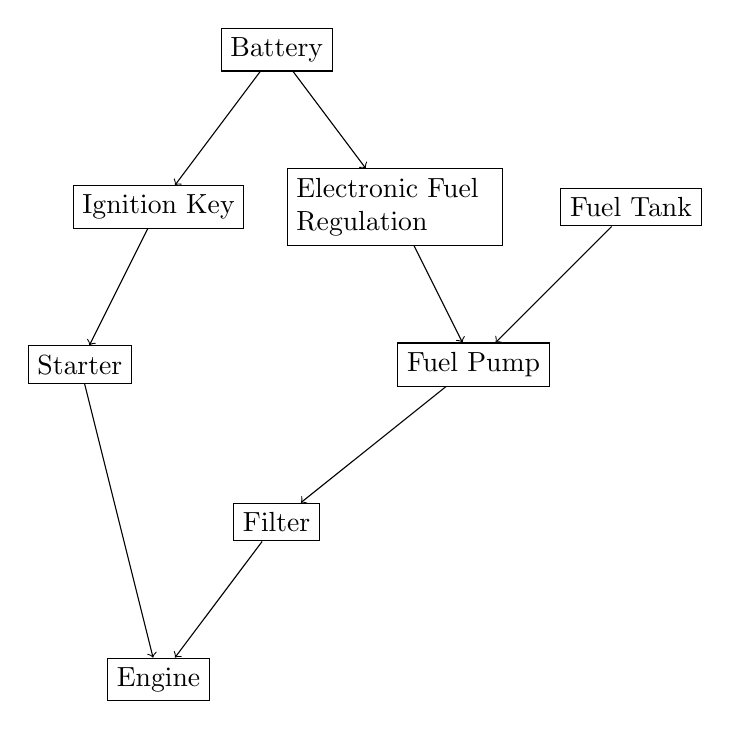
\begin{tikzpicture}
	\node [shape=rectangle,draw=black] (E) at (-1.5,-4) {Engine};
	\node [shape=rectangle,draw=black] (S) at (-2.5,0) {Starter};
	\node [shape=rectangle,draw=black] (F) at (0,-2) {Filter};
	\node [shape=rectangle,draw=black] (FP) at (2.5,0) {Fuel Pump};
	\node [shape=rectangle,draw=black] (FT) at (4.5,2) {Fuel Tank};
	\node [shape=rectangle,draw=black] (I) at (-1.5,2) {Ignition Key};
	\node [text width=2.5cm,shape=rectangle,draw=black] (EFR) at (1.5,2) {Electronic Fuel Regulation};
	\node [shape=rectangle,draw=black] (B) at (0,4) {Battery};
	
	\path [->] (B) edge node {} (I);
	\path [->] (B) edge node {} (EFR);
	\path [->] (I) edge node {} (S);
	\path [->] (S) edge node {} (E);
	\path [->] (FT) edge node {} (FP);
	\path [->] (FP) edge node {} (F);
	\path [->] (F) edge node {} (E);
	\path [->] (EFR) edge node {} (FP); 
\end{tikzpicture}

\begin{align*}
&P(Battery) &&= 0.9\\
&P(\neg Battery) &&= 0.1\\
\end{align*}
\begin{align*}
&P(Ignition Key|Battery) &&= 0.9\\
&P(\neg Ignition Key| Battery) &&= 0.1\\
\end{align*}
\begin{align*}
&P(Electronic Fuel Regulation|Battery) &&= 0.9\\
&P(\neg Electronic Fuel Regulation| Battery) &&= 0.1\\
\end{align*}
\begin{align*}
&P(Fuel Tank) &&= 0.9\\
&P(\neg Fuel Tank) &&= 0.1\\
\end{align*}
\begin{align*}
&P(Starter| Ignition Key) &&= 0.9\\
&P(\neg Starter | Ignition Key) &&= 0.1\\
\end{align*}
\begin{align*}
&P(Fuel Pump | Electronic Fuel Regulation \land Fuel Tank) &&= 0.9\\
&P(\neg Fuel Pump | Electronic Fuel Regulation \land Fuel Tank) &&= 0.1\\
\end{align*}
\begin{align*}
&P(Filter | Fuel Pump) &&= 0.9\\
&P(\neg Filter | Fuel Pump) &&= 0.1\\
\end{align*}
\begin{align*}
&P(Engine | Starter \land Filter) &&= 0.9\\
&P(\neg Engine | Starter \land Filter) &&= 0.1\\
\end{align*}


\end{document}
